\title{Topic 2: Customize Linux Kernel}

\author{Yechang Wu}

%%%%%%%%%%%%%%%%%
% Configuration %
%%%%%%%%%%%%%%%%%

\documentclass[12pt, a4paper, twocolumn]{article}
\usepackage{lipsum}
\usepackage{graphicx}
\usepackage{listings}
\lstset{
  basicstyle=\ttfamily,
  columns=fullflexible,
  frame=single,
  breaklines=true,
  postbreak=\mbox{\textcolor{red}{$\hookrightarrow$}\space},
}

% Any configuration that should be done before the end of the preamble:
\usepackage{hyperref}
\hypersetup{colorlinks=true, urlcolor=blue, linkcolor=blue, citecolor=blue}

\begin{document}

%%%%%%%%%%%%
% Abstract %
%%%%%%%%%%%%

\twocolumn[
  \begin{@twocolumnfalse}
    \maketitle
  \end{@twocolumnfalse}
]

%%%%%%%%%%%
% Article %
%%%%%%%%%%%

\section{Tasks}

\begin{enumerate}
    \item Clone the source code of Linux kernel from the publicly available repo and find the specific kernel version of Ubuntu you installed in Topic 1.
    \item Build the kernel image and replace the original image with the one built by you. Make sure your kernel works well.
    \item Modify the kernel source code and insert some personal marks or logs into the code, then rebuild a kernel image. Show that your marks or logs work well.
    \item Write a two-column report describing your steps to accomplish 1-3 in English with Latex. Make sure your Latex report contains text, table, code snippet, and figure.
    \item Create a directory named "Topic 2" in the repo you created in Topic 1, and submit your code and report to the directory.
\end{enumerate}

\section{Implementations}

\subsection{Task 1}

As shown in listing \ref{lst:fetch}, download linux kernel source code according to the version reported in the result of ``uname'' command.

\begin{lstlisting}[language=bash, caption=Fetch Sources, frame=tlrb, label=lst:fetch]
> uname -r
5.18.17-200.fc36.x86_64
> wget https://cdn.kernel.org/pub/linux/kernel/v5.x/linux-5.18.17.tar.xz
...
'linux-5.18.17.tar.xz' saved [129891768/129891768]
> tar -xJf linux-5.18.17.tar.xz
...
> cd linux-5.18.17 && ls
arch     fs ...
\end{lstlisting}

\subsection{Task 2}

As the listing \ref{lst:build}.


\noindent\begin{minipage}{.45\textwidth}
\begin{lstlisting}[language=bash, caption=Build the kernel,frame=tlrb, label=lst:build]
> cp /boot/config-`uname -r`* .config
> make bzImage -j16
> make modules -j16
> sudo make modules_install
> sudo make install
\end{lstlisting}
\end{minipage}\hfill


\subsection{Task 3}

Then, by adding code in listing \ref{kernel_modifier} to function ``sys\_execve'',
a simple debugging message will appear when ``execve'' syscall triggered.


\noindent\begin{minipage}{.45\textwidth}
\begin{lstlisting}[language=C, caption=Add A Debug Message, frame=tlrb, label=kernel_modifier]
printk(KERN_ALERT "Hello World From The Toy Kernel");
\end{lstlisting}
\end{minipage}\hfill


Rebuild and reinstall the toy kernel, and then reboot to the toy kernel.

The result is as shown in picture \ref{fig:1}.

\begin{figure}
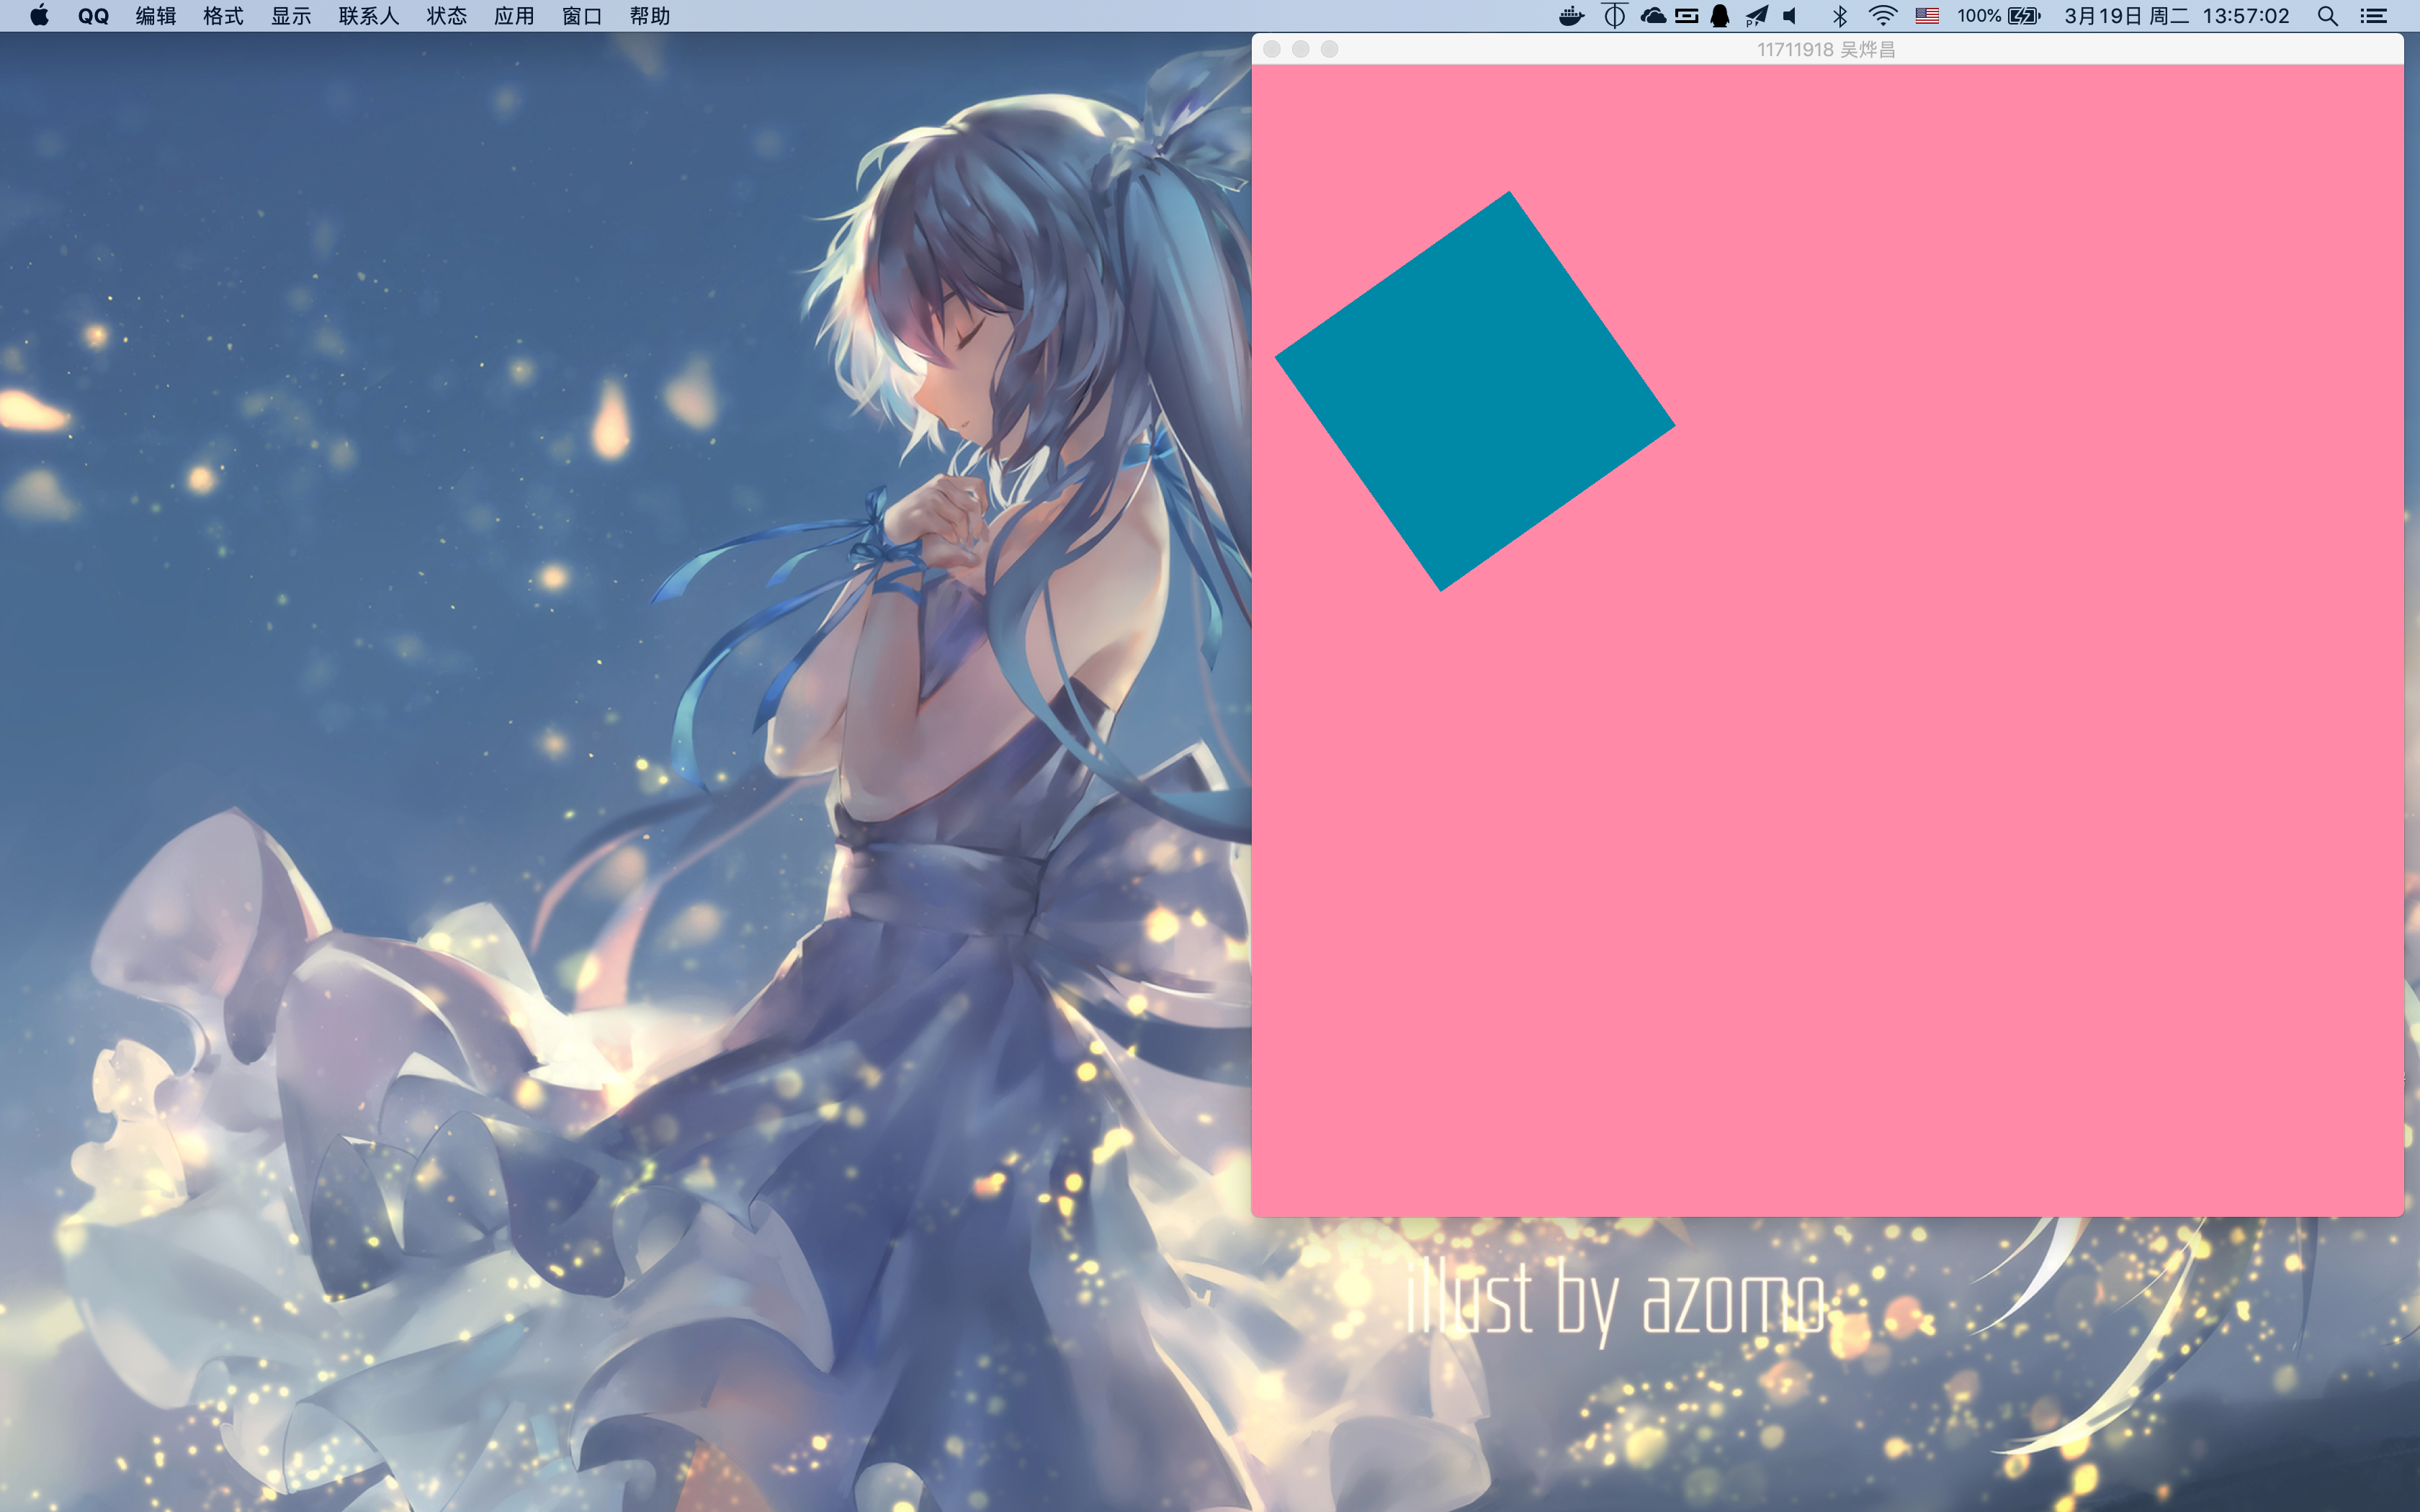
\includegraphics[width=.98\linewidth]{picture/1.jpg}
\caption{Screenshot on logs}
\label{fig:1}
\end{figure}


\end{document}
